\begin{frame}{Biological Analogy}
	\begin{figure}[H]
		\centering
		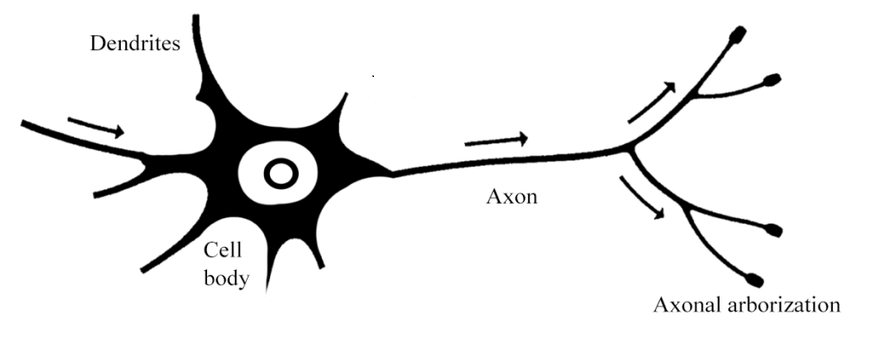
\includegraphics[width=0.9\textwidth]{Figs/biological_neuron.png}
		\caption{Anatomy of a biological neuron \cite{biological-and-nn-neuron}.}
	\end{figure}
\end{frame}

\begin{frame}{Activation Functions}
	\begin{figure}[H]
		\centering
		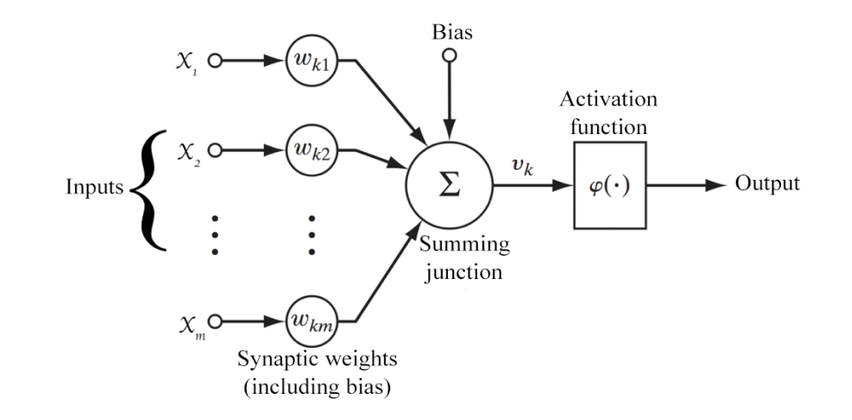
\includegraphics[width=0.9\textwidth]{Figs/nn_neuron.png}
		\caption{Neural network neuron \cite{biological-and-nn-neuron}.}
	\end{figure}
\end{frame}

\begin{frame}{Activation Functions}
	\begin{figure}[H]
		\centering
		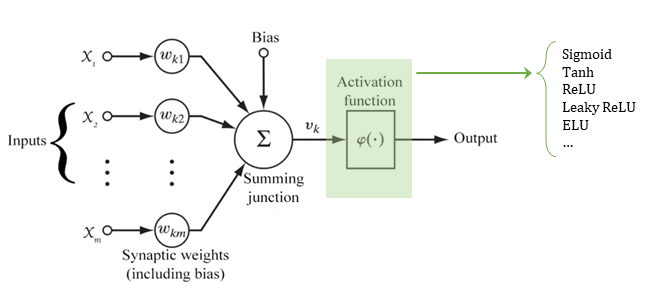
\includegraphics[width=0.9\textwidth]{Figs/activation_function_1.png}
		\caption{Activation function}
	\end{figure}
\end{frame}

\begin{frame}{Activation Functions}
	\begin{figure}[H]
		\centering
		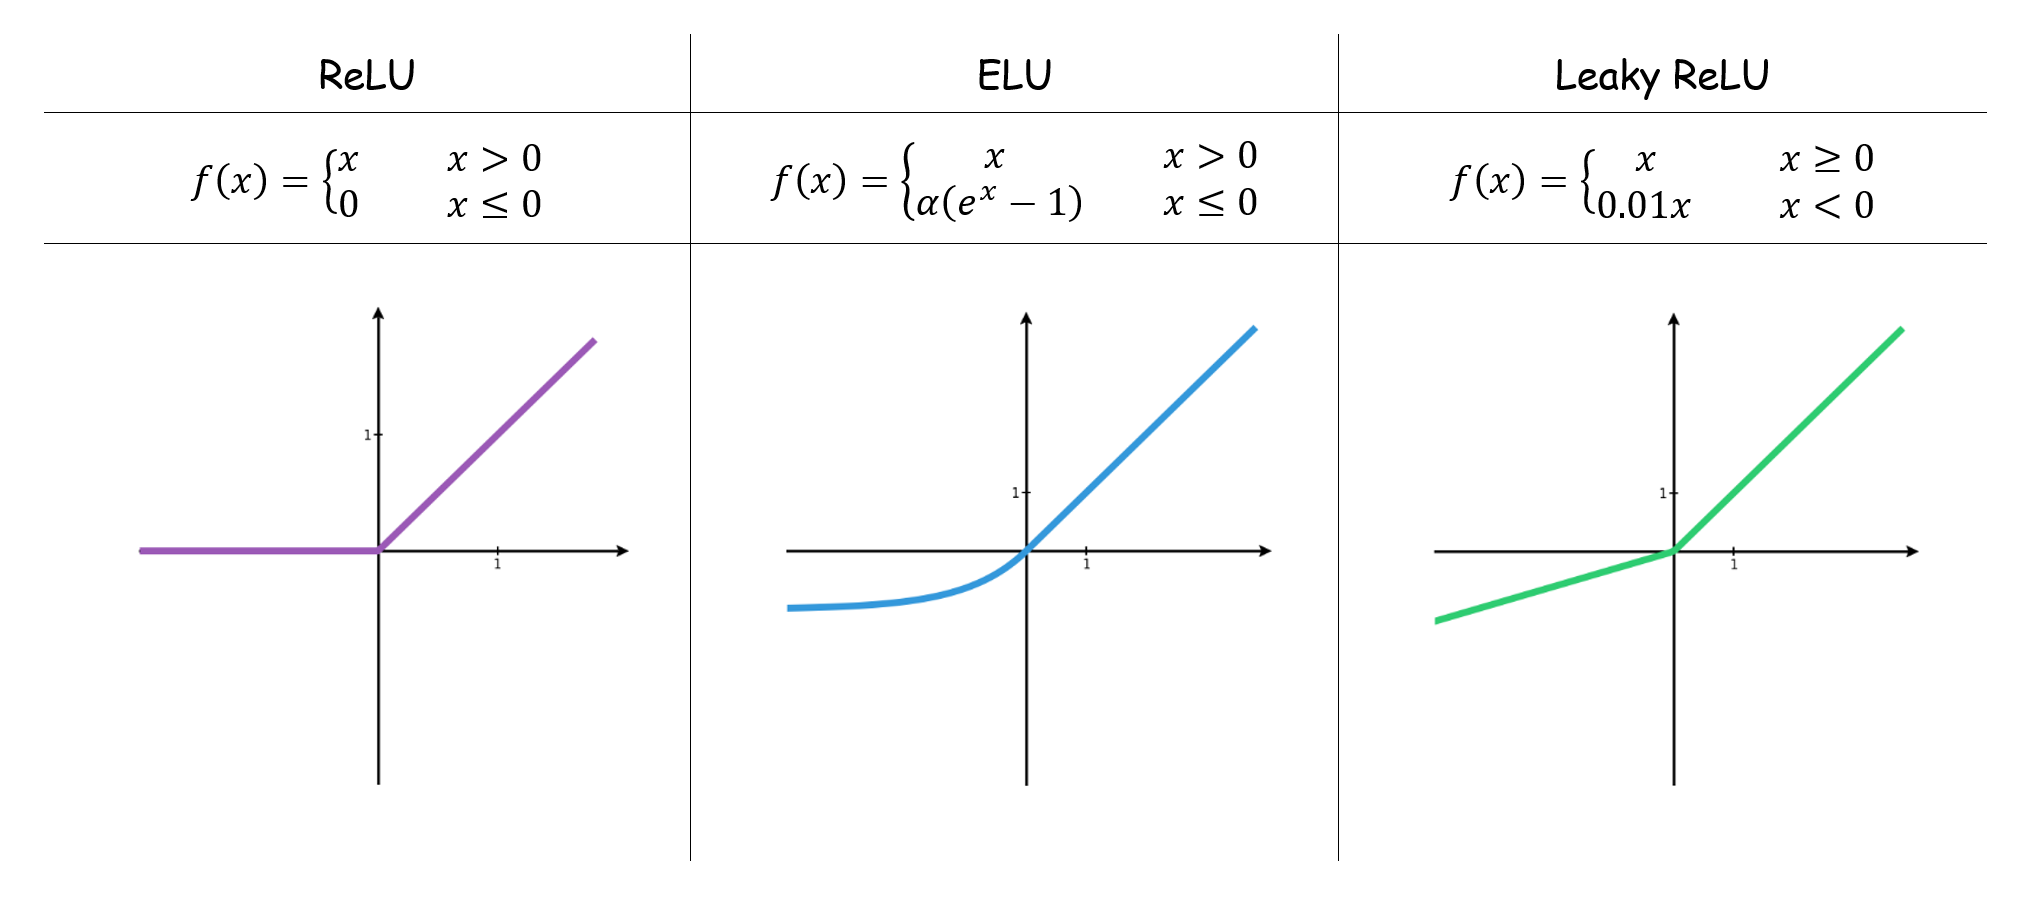
\includegraphics[width=1\textwidth]{Figs/section_1/activation_functions_1.PNG}
	\end{figure}
\end{frame}

\begin{frame}{Activation Functions}
	\begin{figure}[H]
		\centering
		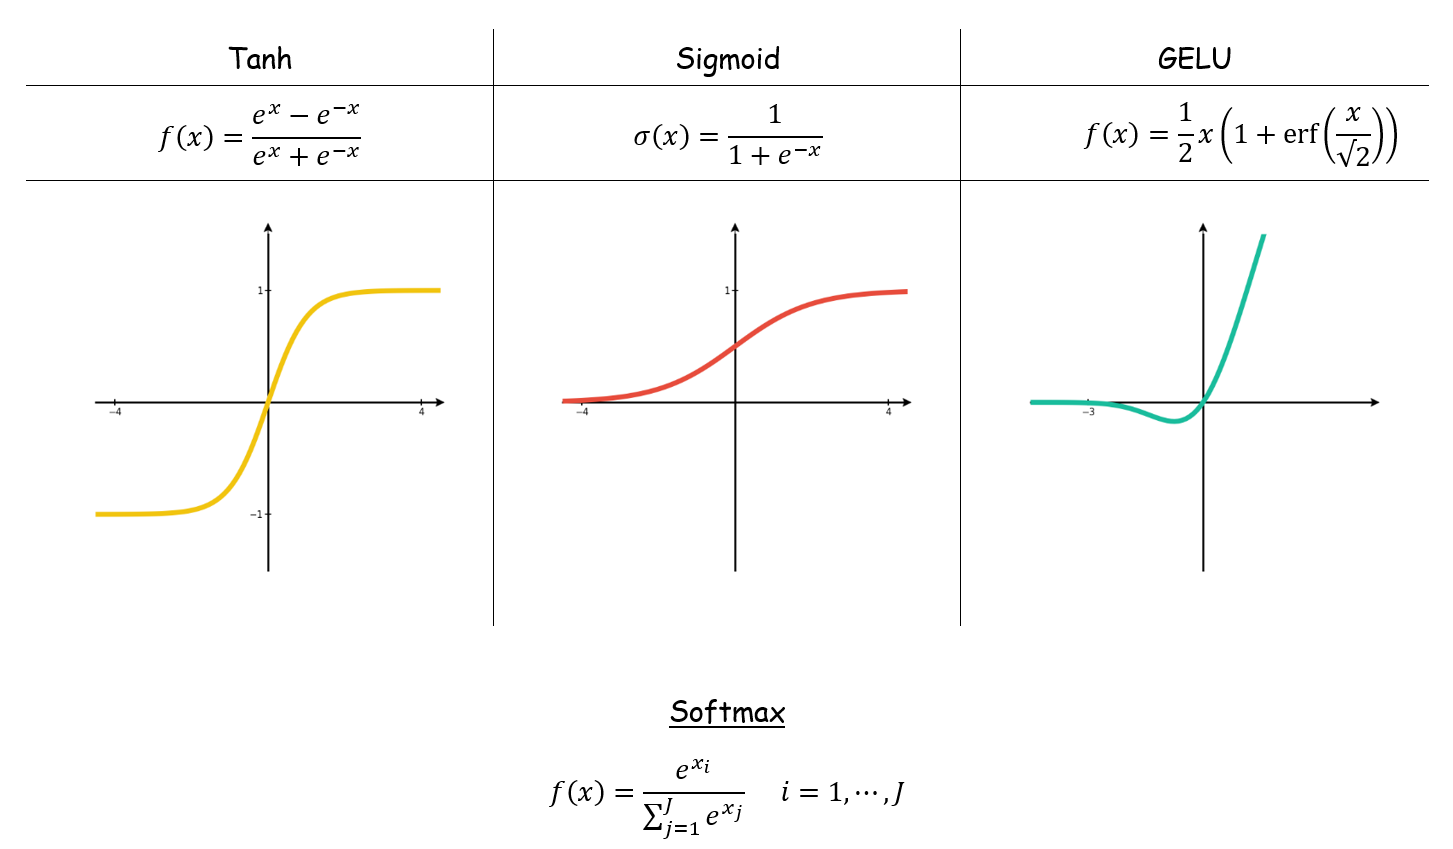
\includegraphics[width=1\textwidth]{Figs/section_1/activation_functions_2.PNG}
	\end{figure}
\end{frame}

\begin{frame}{Gradient Descent}
	\begin{figure}[H]
		\centering
		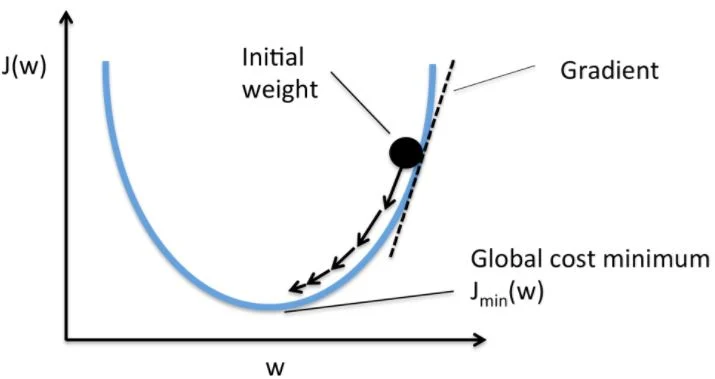
\includegraphics[width=0.70\textwidth]{Figs/gradient_descent2.png}
		\caption{Gradient descent \cite{gradient-descend2}.}
	\end{figure}
\end{frame}